\scanpage{3}

\[
\deleted{\mathrm{N\acute eron}(\unsure{/|1}\quad A\longrightarrow}
\]
\[
\text{\uuline{Néron}}_{A/S}\longrightarrow
\text{\uuline{Hom}}_{S\text{-}\mathrm{gr}}(A,A^*)
\]
\diagram{\begin{tikzcd}[ampersand replacement=\&,column sep=small,row sep=small]
{} \& \overset{s}{A}\times\overset{x}{A}\arrow[d,"\pi"] \& {}\\
(T_s)_*(\xi)-\xi \& A \& x\longrightarrow x-s
\end{tikzcd}}

\[
\deleted{A\mathrel{\unsure{-|\longrightarrow}}D^*}
\]
\[
\unsure{V|\vee}\qquad s\times A\qquad s_*\xi-\xi
\]
% slanted, left of the box
\figure{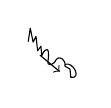
\begin{tikzpicture}[x=.52cm,y=.52cm,line cap=round,line join=round]
\draw (0,0) -- (.05,.32) -- (.12,-.02) -- (.19,.12) -- (.23,-.23) -- (.31,-.12) -- (.33,-.35) .. controls (.44,-.11) and (.52,-.16) .. (.49,-.43) .. controls (.42,-.69) and (.68,-.53) .. (.68,-.45) .. controls (.78,-.32) and (.93,-.48) .. (.90,-.61) -- (1.01,-.67);
\draw[->] (.29,-.34) -- (.77,-.74);
\draw (.91,-.56) .. controls (1.09,-.49) and (1.32,-.92) .. (1.04,-.88) -- (1.02,-.68);
\end{tikzpicture}}

\[
\boxed{\pi^*(\xi)-\mathrm{pr}_1(\xi)-\mathrm{pr}_2(\xi)}
\]

(i) $\xi$ dans le noyau \deleted{$s^*\xi$} de $\text{\uuline{Pic}}_{A/S}^{\deleted{\unsure{\tau}}}\longrightarrow\text{\uuline{Hom}}(A,A^*)$, i.e. $s\xi=\xi$

(i$'$). $\pi^*(\xi)-\mathrm{pr}_1(\xi)-\mathrm{pr}_2(\xi)=0$
\margin{$s.D\sim D$}

(ii) $\xi\in\text{\uuline{Pic}}^\tau_{\deleted{\unsure{A/S}}}(A/S)$

(iii) $\xi\in\mathrm{Im}\,\mathrm{Ext}^{1}_{\deleted{\unsure{S|\xi}}}(A,\mathbb{G}_m)$

$(\mathrm{i})\iff(\mathrm{i}')$ trivial

$(\mathrm{ii})\iff(\mathrm{iii})$ par le raisonnement \inserted{\unsure{géométrique|giraudique}} de Serre

$(\mathrm{ii})\Longrightarrow(\mathrm{i})$ par la propriété additive de $\text{\uuline{Pic}}^\tau$

$(\mathrm{i})\Longrightarrow(\mathrm{ii})$ c'est le th. de Barsotti-Cartier-Serre —

% archive sheet number: 2

